\subsection{Source of Demonstration [MAX 5]}
\label{sec:source_of_demonstration}
Regarding the way how the expert demonstrations can be obtained, according to \cite{fang2019survey}, two categories can be identified: \begin{enumerate*}[label=\textbf{(\alph*)}]
    \item Direct Demonstration. 
    \item Indirect Demonstration.
\end{enumerate*}

\paragraph{Direct Demonstration}  \mbox{} \\
It allows to obtain samples directly from the robot, either with kinesthetic teaching (Figure \ref{fig:kinesthetic}) or teleoperation teaching (Figure \ref{fig:teleoperation}).In kinesthetic teaching the human operator contacts and guides the robot, that collects data by itself, while in teleoperation teaching the human operator remotely guides the robot with joystick, tactile sensor, control panel, and wearable device. 
The former is characterized by the fact that there is no need to consider difference in kinematic between human and robot, as consequence, data has less noise. However, the robot must be passively controllable and require direct contact, introducing safety problems, and unintuitive demonstrations for robot with multiple degrees of freedom.
The latter is characterized by a higher safety, since there is no direct contact, and a wide application range.
A very popular example of teleoperation system is \textit{Roboturk} \cite{mandlekar2018roboturk}, it is a cloud-based teleoperation framework that enables the collection of high-scale demonstration dataset \cite{mandlekar2019scaling,mandlekar2022matters}, for both simulated and real-world robots, using a mobile-phone as controller (Figure \ref{fig:roboturk}). 
While this framework is interesting because it allows to collect data from a wide range of demonstrator with different demonstrations quality, it lacks of tactile information \textcolor{red}{[To continue...]}
 \begin{figure}[htbp]
         \centering
         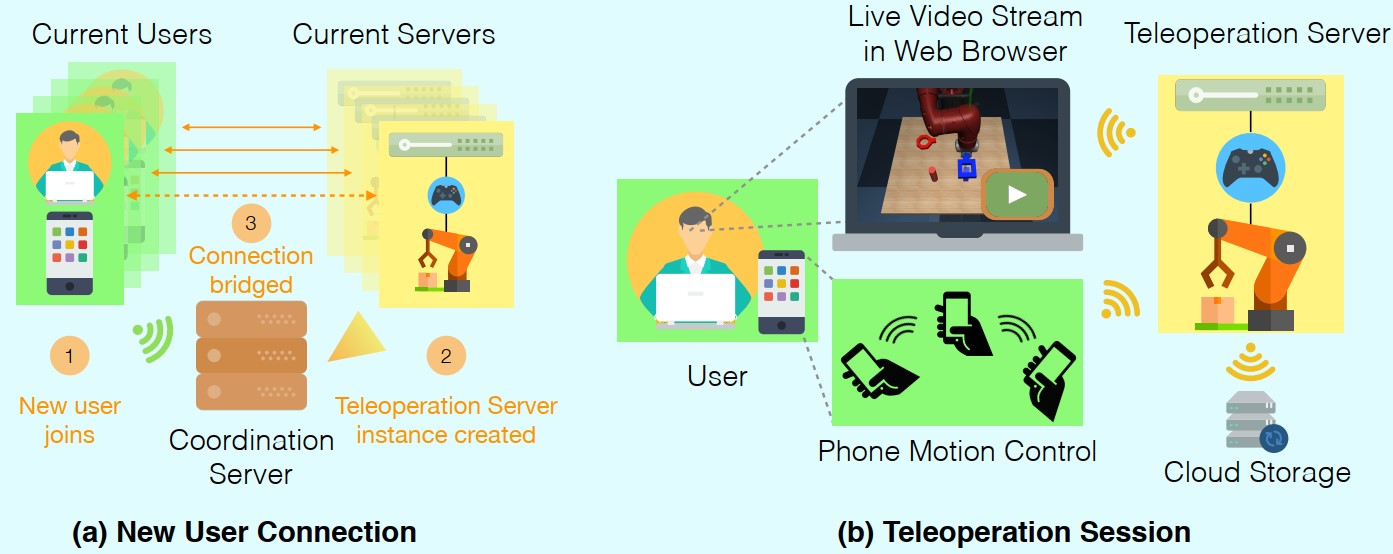
\includegraphics[width=0.8\textwidth]{Figures/images/indirect_demonstration/roboturk.jpg}
         \caption{System diagram of Roboturk \cite{mandlekar2018roboturk}}
         \label{fig:roboturk}
\end{figure}



\paragraph{Indirect Demonstration}  \mbox{} \\ 
It allows samples to be acquired in a way that is completely disconnected from the robotic platform. In this case the human motion is recorded by vision system \cite{} or wearable device \cite{}. In last years, the ability to extrapolate a policy starting from video of human performing a task has become a very important topic in the current literature \cite{fang2019survey,torabi2019recent_advances_lfo}. While Indirect Demonstration based on visual system allows to collect samples in the most intuitive and scalable way possible, potentially any video of performed task can be used, it lacks of relevant information such as the tactile one, moreover, the correspondence problem must be solved, i.e. the system must be able to map motion captured in human space into the corresponding motion of the robot. In Section \ref{sec:lfo} the different way how this problem has been solved in the current literature will be explained in detail. 
\begin{figure}[htb]
     \centering
     \begin{subfigure}[b]{0.45\textwidth}
         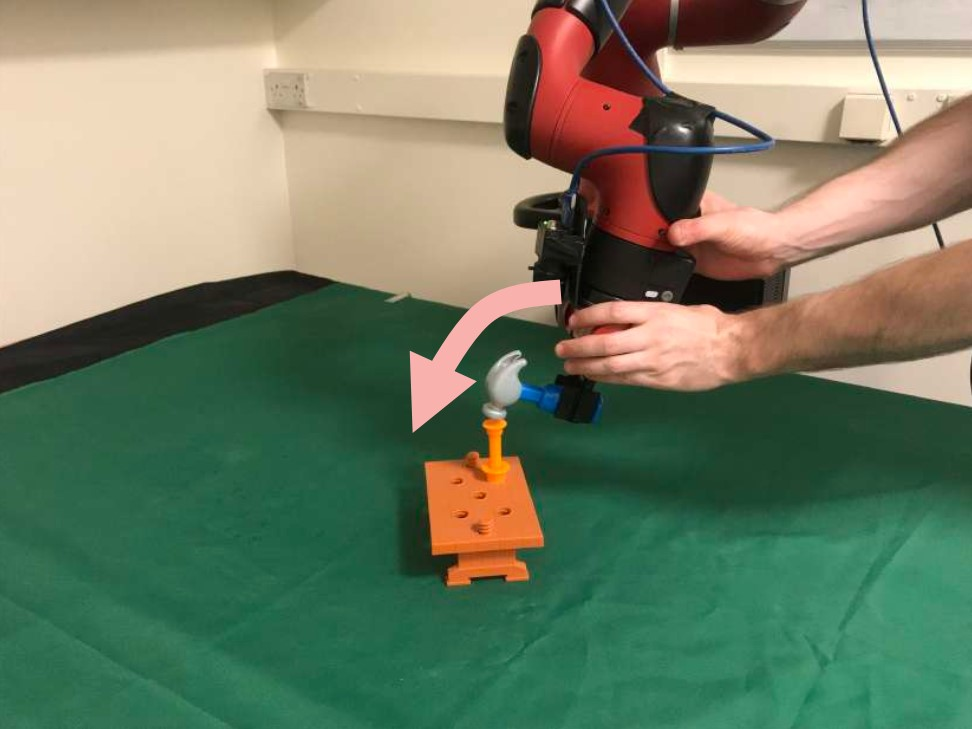
\includegraphics[width=\textwidth]{Figures/images/direct_demonstration/kinesthetic.jpg}
         \caption{Example of kinesthetic teaching \cite{johns2021coarse_to_fine}}
         \label{fig:kinesthetic}
     \end{subfigure}
     \hfill
     \begin{subfigure}[b]{0.5\textwidth}
         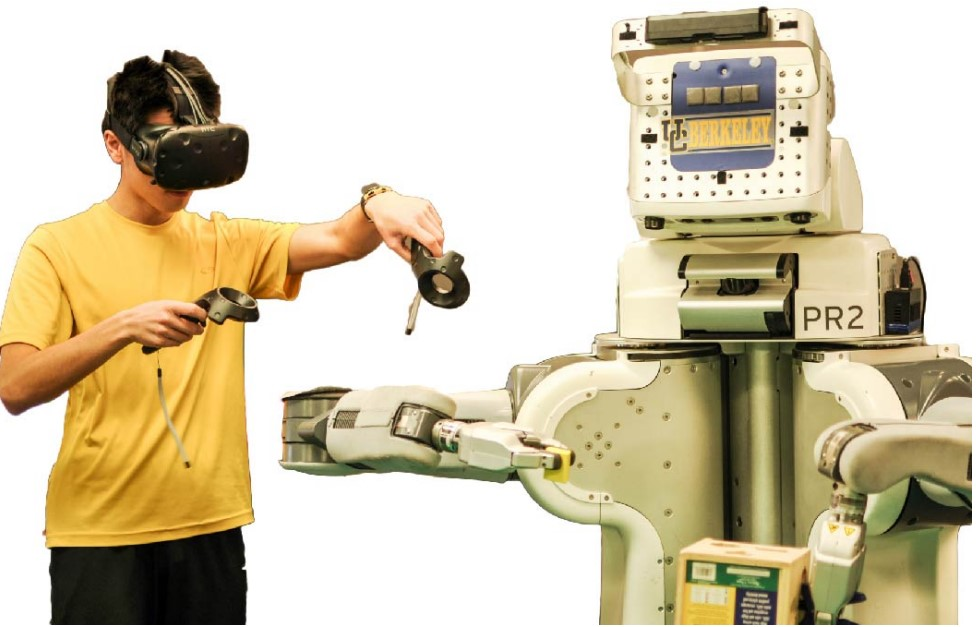
\includegraphics[width=\textwidth]{Figures/images/direct_demonstration/teleoperation.jpg}
         \caption{Example of teleoperation \cite{zhang2018deep_vr_teleoperation}}
         \label{fig:teleoperation}
     \end{subfigure}
    \hfill
    \caption{Examples of Direct Demonstration}
    \label{fig:direct_demonstrations}
\end{figure}

